\begin{htmlonly}
\documentclass{covise}

\usepackage{html, htmllist}
\usepackage{color}
\usepackage{graphicx}
\usepackage{longtable}
\usepackage{palatino}
\usepackage{picins}
\usepackage[colorlinks,dvips]{hyperref}
	  
\bodytext{TEXT=#000000 BGCOLOR=#FFFFFF LINK=#0033CC VLINK=#0033CC}

% #1  mark defined by \label
% #2  a linktext 
% #3  a html link 
\newenvironment{covlink}[3]%
{\html{\htmladdnormallink{#1}{#3}}\latex{\hyperref[#1]{#2} (\ref{#1})}%
}

\newenvironment{covimg}[4]%
{ \html{\htmladdimg[ALIGN=CENTER]{#2.gif}}
 
 \latexonly
 \begin{figure}[!Hhtp]
  \begin{center}
   \includegraphics[scale=#4]{#1/#2}
   \caption{#3}
  \end{center}
 \end{figure}
 \endlatexonly
}



\definecolor{output}{rgb}{0.,0.,1.}
\definecolor{depend}{rgb}{1.,0.65,0.}
\definecolor{required}{rgb}{0.58,0.,0.83}
\definecolor{optional}{rgb}{0.,0.39,0.}

\end{htmlonly}

%================================================================================
%================================================================================


%================================================================================
%\startdocument

\chapter{Proze\ss schritte und Proze\ss ablauf}

\begin{figure}[!Hhtp]
  \begin{center}
   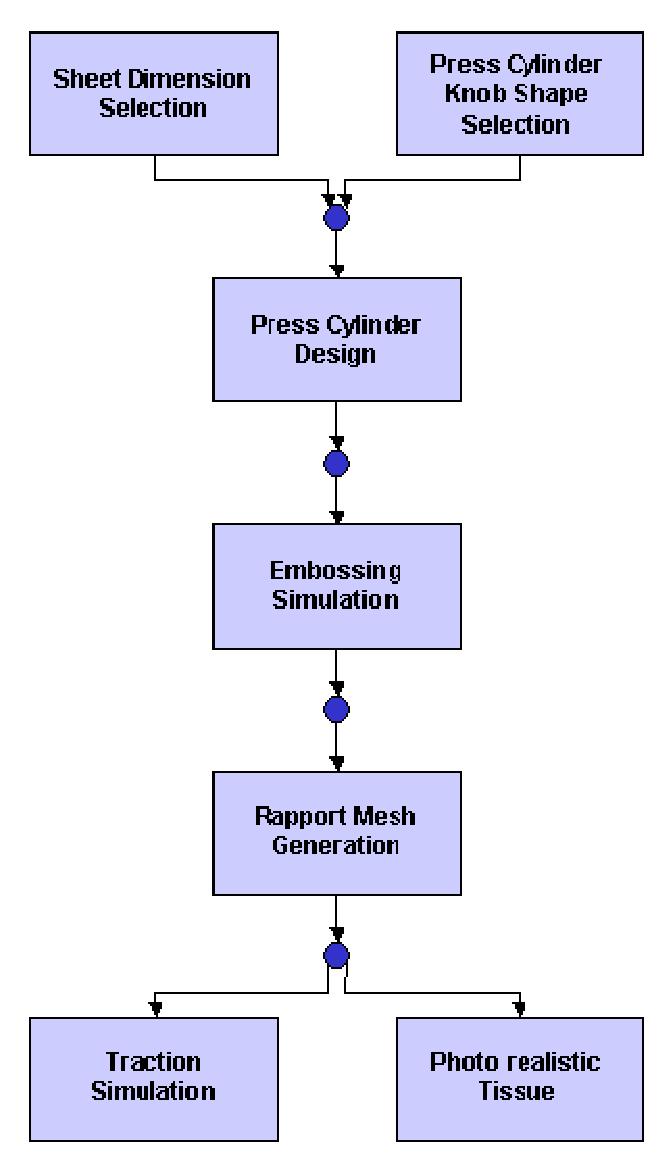
\includegraphics[scale=0.6]{process/flowchart_overview}
   \caption{Flu\ss diagramm}
  \end{center}
\end{figure}

\section{Papiergr\"o\ss e}
Im ersten Schritt muss die Papiergr\"o\ss e festgelegt werden. Es gibt drei
Standardgr\"o\ss en f\"ur Toilettenpapier (engl. Abk\"urzung toipa) und zwei 
Standardgr\"o\ss en f\"ur Haushaltspapier (engl. Abk\"urzung HHT). Au\ss erdem 
gibt es noch die M\"oglichkeit, die Gr\"o\ss e frei einzustellen.

\begin{tabular}{|l|l|l|l|} \hline
Parameter 		& Typ 		& Wertebereich 	& Einheit	\\ \hline
feste Gr\"osse 	& Auswahl 	& Toipa 125x98	& $mm^2$ 	\\ 
				& 		 	& Toipa 140x98	&			\\
				& 		 	& Toipa 125x110&			\\				
				& 			& HHT 246x260	& 			\\ 
			    &			& HHT 246x230	& 			\\ 
				& 			& Custom Dimensions		& 			\\ \hline
variable L\"ange	& Drehknopf	& 100-300 		& $mm$ 		\\ \hline
variable Breite& Drehknopf	& 100-300 		& $mm$ 		\\ \hline
\end{tabular}

Das sichtbare Ergebnis dieses Proze\ss schritts ist eine dreidimensionale
Darstellung des Blattumrisses.

\section{Noppengeometrie der Pr\"agewalze}
Im zweiten Schritt wird die Geometrie des einzelnen Noppen der Pr\"agewalze 
festgelegt. Die Form kann entweder kreisf\"ormig, rechteckig oder elliptisch sein
und wird durch L\"ange und Breite, H\"ohe, Flankenwinkel, Abnutzungsradius
(oben), Ausrundungsradius (Grundradius, unten) und Auslaufzone 
estgelegt. Die Auslaufzone wird vorerst fest auf 1 mm eingestellt.
L\"ange, Breite, H\"ohe, Flankenwinkel, Abnutzungsradius
(oben) und Ausrundungsradius (Grundradius, unten) sind Parameter; im Fall eines
Kreises bedeutet L\"ange = Breite = Durchmesser, im Fall einer Ellipse L\"ange
= gro\ss e Achse, Breite = kleine Achse.

\begin{figure}[!Hhtp]
  \begin{center}
   \includegraphics[scale=0.7]{process/knob_new}
   \caption{Noppengeometrie}
  \end{center}
\end{figure}

Da mit dieser Noppengeometrie das Tissue gepr\"agt wird und daf\"ur u. U.
eine Simulation notwendig ist, ist es f\"ur den
Benutzer jetzt schon wichtig zu wissen, ob f\"ur diese Geometrie 
in der Datenbank Simulationsergebnisse vorhanden sind. Als Ergebnis
der Suche wird eine Liste der \"ahnlichen Noppen aus der Datenbank
geliefert, in der man den im folgenden zu verwendenden Noppen ausw\"ahlen muss.
Die Kriterien f\"ur \"ahnlich sind als erstes die Noppenform und danach alle
Noppen dieser Form, die in den anderen Kriterien nicht mehr als 10 \% abweichen.

\vspace{0.5cm}
\begin{tabular}{|l|l|l|l|} \hline
Parameter 			& Typ 		& Wertebereich 	& Einheit	\\ \hline
Shape (Form) 			& Auswahl 	& Kreis, Ellipse, Rechteck &	\\ \hline		
Length (L\"ange)  	        & Drehknopf & 0.4-5.0	& $mm$ 		\\ \hline
Width (Breite)	            	& Drehknopf & 0.4-5.0	& $mm$ 		\\ \hline
Height (H\"ohe)				& Drehknopf	& 100-300 		& $mm$ 	\\ \hline
Flank Angle (Flankenwinkel)		& Drehknopf	& 0.0-35.0 		& $\symbol{23}$ 		\\ \hline
Abrasion Radius (Abnutzungsradius)	& Drehknopf	& 0.0-0.5 		& $mm$ 		\\ \hline
Ground Radius (Ausrundungsradius)	& Drehknopf	& 0.0-0.5 		& $mm$ 		\\ \hline
Data Base (Datenbanksuche)		& Auswahl	& siehe unten   &			\\ \hline
\end{tabular}
\vspace{0.5cm}



Die Liste der \"ahnlichen Noppen sieht jedesmal anders aus, dies
hier ist ein Beispiel:
\begin{itemize}
\item my Knob (not) in DB (h=2.0 l=0.4 b=0.4 a=20 ra=0.5 rg=0.5)
\item similar Knob in DB (h=2.0 l=0.4 b=0.4 a=20 ra=0.5 rg=0.5)
\item similar Knob in DB (h=2.0 l=0.4 b=0.4 a=20 ra=0.5 rg=0.5)
\end{itemize}


Wenn ein anderer als der \"uber die Parameter eingestellte Noppen
gew\"ahlt wird, passen sich die Parameter automatisch an.

Das sichtbare Ergebnis dieses Proze\ss schritts ist eine dreidimensionale
Darstellung des Noppen, die aus wenigen Polygonen besteht. 

\section{Design des Pr\"agemusters}
Im dritten Schritt wird das Muster festgelegt. Es gibt zwei M\"oglichkeiten:
parametrisches oder freies Design des Musters. In beiden F\"allen werden
dadurch die Positionen der Noppen auf dem Rapport festgelegt.

Das sichtbare Ergebnis dieses Proze\ss schritts ist eine dreidimensionale
Darstellung des Musters auf einem Blatt. Der Rapport wird daf\"ur so oft 
wiederholt, dass er ein Blatt ausf\"ullt. F\"ur die Darstellung des Noppens
wird die Geometrie eines Walzennoppens genommen, man sieht also den
Walzenzylinder abgewickelt auf ein Blatt.

W\"ahrend das Design entworfen wird, wird st\"andig
gepr\"uft, ob f\"ur dieses Design sp\"ater eine Zugsimulation m\"oglich ist. 
F\"ur eine Simulation m\"ussen n\"amlich sp\"ater die einzelnen Noppen zu
einem Gesamtgitter vernetzt werden. Dies geht nur dann, wenn sich die
Noppen samt ihrer Auslaufzone nicht zu nahe kommen oder gar durchdringen. 
({\it Kriterium f\"ur zu nahe: Auslaufzonen benachbarter Noppen \"uberschneiden sich})
Deshalb wird der
Umriss der Fu\ss fl\"ache zus\"atzlich dargestellt. Die Umrisslinie
ist blau, solange das Design in Ordnung ist, sie wird gelb, wenn die
Noppen sich zu nahe kommen. 

\subsection{Parametrisches Design}
Parametrisch bedeutet, dass das Muster durch einige wenige Parameter 
festgelegt wird. Damit kann man leicht einfache Grundpr\"agungen erzeugen,
bei denen die Noppen entlang einer Geraden plaziert werden. Man gibt den
Winkel der Geraden zum Rand hin an und den Abstand der Noppen auf der Geraden.
Der Rapport passt sich beim parametrischen Design automatisch so an, dass
er von zwei auf einer Gerade liegenden Noppen jeweils ein Viertel enth\"alt.
Das Gesamtmuster entsteht durch Replizieren (Versetzen) des Rapports. 
Die Orientierung des Rapports \"andert sich dadurch nicht.
 
\begin{figure}[!Hhtp]
  \begin{center}
   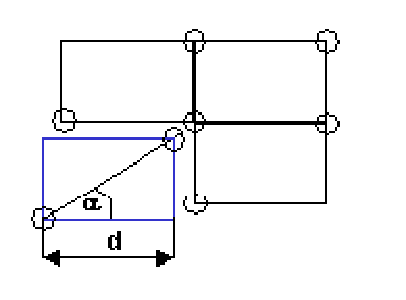
\includegraphics[scale=0.7]{process/pdesign}
   \caption{Parametrisches Design}
  \end{center}
\end{figure}

\begin{tabular}{|l|l|l|l|} \hline
Parameter 		& Typ 		& Wertebereich 	& Einheit		\\ \hline
Winkel			& Drehknopf	& 0.0-90.0 		& \symbol{23}	\\ \hline
Abstand 		& Drehknopf	& 10.0-0.7 		& $mm$ 			\\ \hline
\end{tabular}


\subsection{Freies Design}
Beim freien Design k\"onnen die Noppenpositionen von einer Datei eingelesen 
und dann noch interaktiv ver\"andert werden. Die L\"ange und Breite des Rapports
kann frei eingestellt werden. Damit lassen sich komplexe Muster erzeugen.

\begin{figure}[!Hhtp]
  \begin{center}
   \includegraphics[scale=0.7]{process/fdesign_new}
   \caption{Freies Design}
  \end{center}
\end{figure}


Die Datei ist ascii und sieht folgenderma\ss en aus:
\begin{samepage}
\begin{verbatim}
20.0 20.0

11

 8.0  0.0
 5.0  5.0
 0.0  8.0
20.0  0.0
15.0  5.0
10.0 10.0
 5.0 15.0
 0.0 20.0
20.0 12.0
15.0 15.0
12.0 20.0
\end{verbatim}
\end{samepage}

In der ersten Zeile steht die Rapportgr\"o\ss e in mm, in der zweiten Zeile die
Anzahl der Punkte und in den folgenden Zeilen jeweils die x- und y-Position
der Punkte bezogen auf die linke untere Ecke des Rapports.

\vspace{0.5cm}
\begin{tabular}{|l|l|l|l|} \hline
Parameter 		& Typ 		& Wertebereich 	& Einheit		\\ \hline
Rapportl\"ange	& Drehknopf	& siehe unten		& $mm$			\\ \hline
Rapportbreite 	& Drehknopf	& siehe unten		& $mm$ 			\\ \hline
\end{tabular}
\vspace{0.5cm}

Der erlaubte Wertebereich f\"ur Rapportl\"ange und -breite wird der f\"ur die Visualisierung
benutzten COVISE-Map entnommen. Im Augenblick steht dort ein Intervall 2-20 oder 2-30, aber
vermutlich sollten diese Werte auf Grund von Erfahrungen mit dem Modell modifiziert werden.
\newline
\newline
Bitte beachten:
\begin{itemize}
\item Die Benutzerschnittstelle (COVER) erlaubt es, Werte innerhalb des in der Map
vorgegebenen Wertebereichs zu spezifizieren.
\item Um diesen Wertebereich zu erweitern, muss die Map modifiziert werden (siehe Kapitel
3.10 - Modul ControlSCA)
\end{itemize}  

Das interaktive \"andern der Noppenpositionen ist als direkte Manipulation
implementiert, d. h. der Noppen wird mit dem dreidimensionalen Eingabeger\"at
ausgew\"ahlt und bewegt.

\section{Pr\"agesimulation}
Bei der realen Pr\"agung wird das Tissue auf eine Gummiunterlage gelegt
und mit der Metallwalze gepr\"agt. In der Simulation muss die Verformung
in diesen drei Teilen (Gummi, Tissue, Metall) berechnet werden. 
Eine numerische Simulation funktioniert so, dass die Bereiche, in denen 
die Verformung berechnet wird, in Zellen zerlegt werden und dann die 
Verformungsgleichungen f\"ur diese Zellen gel\"ost werden. Die Zerlegung
in Zellen wird als Gittergenerierung bezeichnet und ist nur schwer
automatisierbar, weil die Zellengr\"o\ss e entsprechend den erwarteten
Verformungen angepasst werden muss (an Stellen mit geringer Verformung kann
man mit grossen Zellen rechnen, bei starker Verformung braucht man
kleinere Zellen). Das Gitter enth\"alt deutlich mehr Zellen als die
Geometrie (die f\"ur die Design-Darstellung ben\"otigt wird).
Die Form der Zellen beeinfl\"usst zudem noch die G\"ute
des Rechenergebnisses, die Winkel einer Zelle sollten nicht zu spitz
werden. Da die Noppengeometrie aber auf rechteckige und elliptische
Noppen festgelegt ist und die Problembereiche daher bekannt sind, konnte 
in diesem Projekt ein automatischer Gittergenerierer entwickelt werden.

Das Tissue und das Metallteil (eines Viertel-Noppens) werden in 
zweidimensionale Zellen zerlegt, da der Gummi sich stark verformt, 
muss er in dreidimensionale Zellen zerlegt werden.

Dann muss der Benutzer noch das Tissue-Material festlegen, er kann dabei aus
sechs Materialien ausw\"ahlen. Desweiteren muss der Anpressdruck und die
Gummih\"arte eingestellt werden.

Aus diesen Daten wird die Eingabedatei f\"ur die Simulation erzeugt. 
Jetzt erst kann die eigentliche Pr\"agesimulation gestartet werden. Daf\"ur
wird das Programm LS-Dyna verwendet. Das Ergebnis der Simulation ist das
Gitter des verformten Tissue f\"ur einen Noppen und Spannungen bzw. 
Verformungen in den Gitterzellen.

Da die Gittergenerierung und die Simulation viel Zeit brauchen, werden
die Ergebnisse in einer Datenbank abgelegt. Sobald der Benutzer Tissuetyp,
Gummih\"arte und Anpressdruck gew\"ahlt hat, wird gepr\"uft, ob es f\"ur
diese oder \"ahnliche Parameter schon 
Simulationsergebnisse gibt und diese als Liste zur Verf\"ugung gestellt. Wenn
sich der Benutzer f\"ur Parameter aus der Datenbank entscheidet, wird
bei Simulationsstart gar keine Simulation gemacht, sondern nur die
Ergebnisse aus der Datenbank geholt.

\vspace{0.5cm}
\begin{tabular}{|l|l|l|l|} \hline
Parameter 		& Typ 		& Wertebereich 	& Einheit	         \\ \hline
Rubber Hardness (Gummih\"arte) 	& dial		& s. Anm. 1 	& \symbol{23} $Shore$ \\ \hline
Contact Pressure (Anpressdruck)	& dial		& s. Anm. 2 	& $N per knob$ 	 \\ \hline
Tissue Type      	& Auswahl 	& TAD		&		 \\ 
			& 		& Slush 	&		 \\
			& 		& Double Velvet &		 \\				
			& 		& HHT Convent	& 		 \\ 
			&		& HHT      	& 		 \\ 
			& 		& BSQ A 	& 		 \\ \hline
Data Base (Datenbankergebnisse)		& Auswahl	& s. Anm. 3	& - 		 \\ \hline
Start Embossing (Starte Simulation)    	& Boolean   	& -             & -              \\ \hline
\end{tabular}
\vspace{0.5cm}


Anmerkungen: 
\begin{enumerate}

\item Im Augenblick wird der angegebene Wert f\"ur Gummih\"arte ignoriert (ausgenommen dass er
in der Datenbank gespeichert wird) und die Simulation wird mit vordefinierten Werten
gestartet.

\item Anpressdruck bedeutet genau die maximale Kraft {\bf pro Noppen}. Dieser Wert kann
innerhalb des durch die Map definierten Wertebereichs modifiziert werden. Die Werte in der
Map m\"ussen u. U. entsprechend den Erfahrungen mit dem Modell angepasst werden.
  
\item Durchsuchen der Datenbank bedeutet: Zuerst wird nach dem selben Material gesucht,
danach werden alle Noppen aufgelistet, die bez\"uglich der Gummih\"arte und des Anpressdrucks
maximal 10 \% abweichen.\newline 
Die Liste sieht etwa folgendermassen aus:
	\begin{itemize}
	\item my knob in DB (p=100 h=50)
	\item my knob (not) in DB
	\item similar knob in DB (p=100 h=50)
	\item similar in DB (p=100 h=50)
	\end{itemize}
\end{enumerate}

Das visuelle Ergebnis der Pr\"agesimulation ist eine dreidimensionale
Darstellung des gepr\"agten Noppen.

\section{Vernetzung aller Noppen im Rapport}
F\"ur die photorealistische Darstellung und die Zugsimulation m\"ussen
alle Gitter der gepr\"agten (verformten) Noppen innerhalb des Rapport zu einem 
Gesamtgitter verbunden werden. Daf\"ur wird das Programm Ansys verwendet.

Diese Vernetzung wird automatisch nachdem die Verformung berechnet oder aus
der Datenbank ausgelesen wurde, gestartet. Dieser Schritt ist fuer den
Benutzer nicht sichtbar, es gibt dafuer auch kein visuelles Ergebnis.

\section{Photorealistische Darstellung}
Die photorealistische Darstellung erreicht man dadurch, dass man eine
Textur (ein digitales Bild) des ungepr\"agten Tissue auf das verformte
Gitter des Rapport legt. In dem Bild muss die Papierstruktur gut zu
erkennen sein, es muss so hoch aufgel\"ost sein, dass auch aus geringer 
Entfernung einzelne Pixel nicht erkennbar sind. Da der Rapport mehrmals
aneinandergesetzt wird, ist eine gleichm\"a\ss ige Farbe und Beleuchtung
wichtig. 

Es gibt zwei Darstellungsarten: als Blatt und als Rolle. In beiden F\"allen
muss der Rapport vervielfacht werden. Da das Gitter eines verformten
Noppen aus relativ vielen Zellen besteht, besteht das Blatt oder die
Rolle aus so vielen Zellen, dass die Frame-Rate (Rate mit der ein
neues Bild gezeichnet wird), stark absinkt.

\vspace{0.5cm}
\begin{tabular}{|l|l|l|l|} \hline
Parameter 	& Typ 		& Wertebereich 	& Einheit	\\ \hline
Darstellungsart	& Auswahl	& Rolle 	& -		\\ 
		&	 	& Blatt		& -		\\ \hline
\end{tabular}
\vspace{0.5cm}

Das Ergebnis dieses Schritts ist die photorealistische Darstellung als
Blatt oder als Rolle. In der Rollendarstellung werden auch noch
die Stirnseiten und die innere Papprolle dargestellt.

\section{Zugsimulation}
Beim realen Zugversuch w\"urde man ein Blatt Tissue mit einer bestimmten
Kraft auseinanderziehen und messen, bei welcher Kraft es reisst.\newline
\newline 
In der Simulation ermittelt man die Verformungen innerhalb eines Rapports.
\newline
Die endg\"ultige Version (noch nicht implentiert) soll folgenderma\ss en aussehen:\newline
Die maximale Wert f\"ur die Deformation des Rapports und die Anzahl der Schritte bis zum
Erreichen dieses Zustands werden vorgegeben. Dann wird Schritt f\"ur Schritt simuliert.
Zus\"atzlich wird der prozentuale Verlust berechnet und als Zahl ausgegeben.\newline
\newline
Aktuelle Implementierung:\newline
Die Zugsimulation berechnet, grob formuliert, ein Mass f\"ur die Verformung. Genauer
gesagt: Das Programm berechnet die von-Mises-Spannung f\"ur die Gitterzellen. Diese Werte
sind ein Mass f\"ur die "Inhomogenit\"at" (bez\"uglich Richtung und St\"arke) der auf die Gitterzellen
innerhalb des Rapports wirkendenden Kr\"afte: Je h\"oher der Wert umso wahrscheinlicher
kann das Papier an dieser Stelle reissen.\newline
\newline
In jedem Fall werden die entsprechenden Eingabedateien f\"ur Ansys erzeugt und die
Simulation gestartet. Im Fall der aktuellen Implementierung wird die von-Mises-Spannung
an den Gitterzellen berechnet als Mass f\"ur eine m\"ogliche Deformation und in Farben
umgesetzt (blau: schwache Verformung, rot: starke Verformung)


%\begin{tabular}{|l|l|l|l|} \hline
%Parameter 		& Typ 		& Wertebereich 	& Einheit		\\ \hline
%Zugkraft		& Drehknopf	& ? 			& $N/mm^2$		\\ \hline
%\end{tabular}

Das sichtbare Ergebnis ist dann eine dreidimensionale Darstellung
des Rapports als Polygonmodell mit Farben. 

%Desweiteren wird der Verlust in Prozent ermittelt und als Zahl
%ausgegeben.
